\documentclass{article}
\usepackage{ctex,circuitikz,geometry,graphicx,amsmath,amssymb,amsthm,subcaption,appendix,hyperref}
\usepackage{listings}
\usepackage{xcolor}
\lstset{
    basicstyle=\tt,
    keywordstyle=\color{purple}\bfseries,
    identifierstyle=\color{brown!80!black},
    commentstyle=\color{gray}
    showstringspaces=false,
    numbers=left, 
    breaklines=true,
    numberstyle= \tiny, 
    keywordstyle= \color{ blue!70},
    commentstyle= \color{red!50!green!50!blue!50}, 
    frame=shadowbox, % 阴影效果
    rulesepcolor= \color{ red!20!green!20!blue!20} ,
    escapeinside=``, % 英文分号中可写入中文
    xleftmargin=2em,xrightmargin=2em, aboveskip=1em,
    framexleftmargin=2em
} 
\geometry{a4paper,scale=0.8}
\ctikzset{american,european resistors}
\ctikzset{tripoles/mos style/arrows}
\ctikzset{tripoles/pmos style/nocircle}
\title{《电子系统综合设计与制作》课程设计报告\\——\textit{智能磁阻式电磁炮台}}
\author{江玮陶\quad 2023010631\\张光宇\quad 2023010629\\陈冠嘉\quad 2023010503}
\begin{document}
\maketitle
\tableofcontents
\section{项目背景}
电磁炮是指使用电磁力发射炮弹的新型发射装置,其原理的提出已很久远,至少有近百年历史。随着脉冲电源技术的成熟和电脑仿真技术的出现,电磁炮技术自上世纪70年代起开始出现突破性进展,在学术和军事领域展现重要的潜在应用前景。

电磁炮从原理上分为线圈炮和轨道炮,前者又可以按照磁力的来源分为磁阻炮和感应炮两种。磁阻炮的加速原理类似级联的电磁铁,通过精巧的控制各级线圈的通电时机达到“接力”加速弹丸的目的,由于其结构简单、可拓展性强且不依赖急剧变化的电流,本项目采取多级磁阻作为炮体部分。
\section{项目简介}
本项目具有如下功能:
\begin{itemize}
    \item 基于半桥拓扑的线圈驱动功能: 采用半桥电路驱动线圈,实现高效能量传输和能量回收,提高电磁炮的效率和性能。
    \item 基于\texttt{Arduino Mega}、舵机云台的瞄准功能: 利用\texttt{Arduino Mega}控制舵机云台,实现目标的自动瞄准和跟踪。
    \item 基于部署在\texttt{K210}端侧计算平台的\texttt{YOLO2}模型的人体识别功能: 利用K210强大的计算能力,部署\texttt{YOLO2}模型进行人体识别,并返回目标位置和大小信息。
\end{itemize}
\section{子模块设计与实现}
\subsection{基于ZVS的升压电路}
为了给电磁炮提供足够的能量,本项目采用ZVS充电器电路进行线圈充电。该电路利用变压器和功率开关,将低压直流电转换为高压直流电,并为线圈提供能量。为了提高电路的可靠性和安全性,本项目采用带隔离控制的升压器,避免高压对控制电路的影响。
\begin{figure}
    \centering
    \begin{minipage}[b]{0.9\linewidth}
        \centering
    \begin{circuitikz}
        \draw (0,0) to[R=$R_2$,l_=$470\Omega$] (2,0);
        \draw(0,4) to [R=$R_3$,l^=$470\Omega$](2,4);
        \draw(2,4) to [R,l_=$10k\Omega$](2,2);
        \draw(2,0) to [R,l^=$10k\Omega$](2,2);
        \draw(2,2) to[short,*-](4,2);
        \draw(4,2) to[short,*-*](8.98,2);
        \draw(4,2) to[full Zener diode,l^=$1N4467$](4,4);
        \draw(4,2) to[full Zener diode,l_=$1N4467$](4,0);
        \draw(3,2)node[ground]{};
        \draw(2,4)to[short](8,4);
        \draw(2,0)to[short](8,0);
        \draw(8,4)node[nmos,anchor=G](Q1){};
        \draw(8,0)node[nmos,anchor=G,yscale=-1](Q2){};
        \draw(Q1.base)node[anchor=south]{Q1};
        \draw(Q2.base)node[anchor=south]{Q2};
        \draw(Q1.source)to[short](Q2.source);
        \draw(0,0)to[short](0,6);
        \draw(0,6)node[vcc]{12V};
        \draw(5.2,0)to[D,l_=$FR107$,*-](5.2,5);
        \draw(7,4)to[D,l_=$FR107$,*-](7,-1);
        \draw(11,4.1)node[transformer core,anchor=base,yscale=2](T){};
        \draw(T.B1)node[circ]{ACout};
        \draw(T.B2)node[circ]{ACout};
        \draw(5.2,5)to[short] (9.95,5);
        \draw(9.95,5)to[short](T.A1);
        \draw(7,-1)to[short](9.95,-1);
        \draw(9.95,-1)to[short](T.A2);
        \draw(Q1.drain)to[short](8.98,5);
        \draw(Q2.drain)to[short](8.98,-1);
        \draw(10.6,2)to[short,*-](9.5,2);
        \draw(9.5,2)to[short](9.5,6);
        \draw(0,6)to[L=$100\mu H$](9.5,6);
        \draw(T.B1)to[open,european,v^=$hv$](T.B2);
        \end{circuitikz}
    \end{minipage}
    \\
    \hspace{20pt}
    \\
    \begin{minipage}[b]{.45\linewidth}
        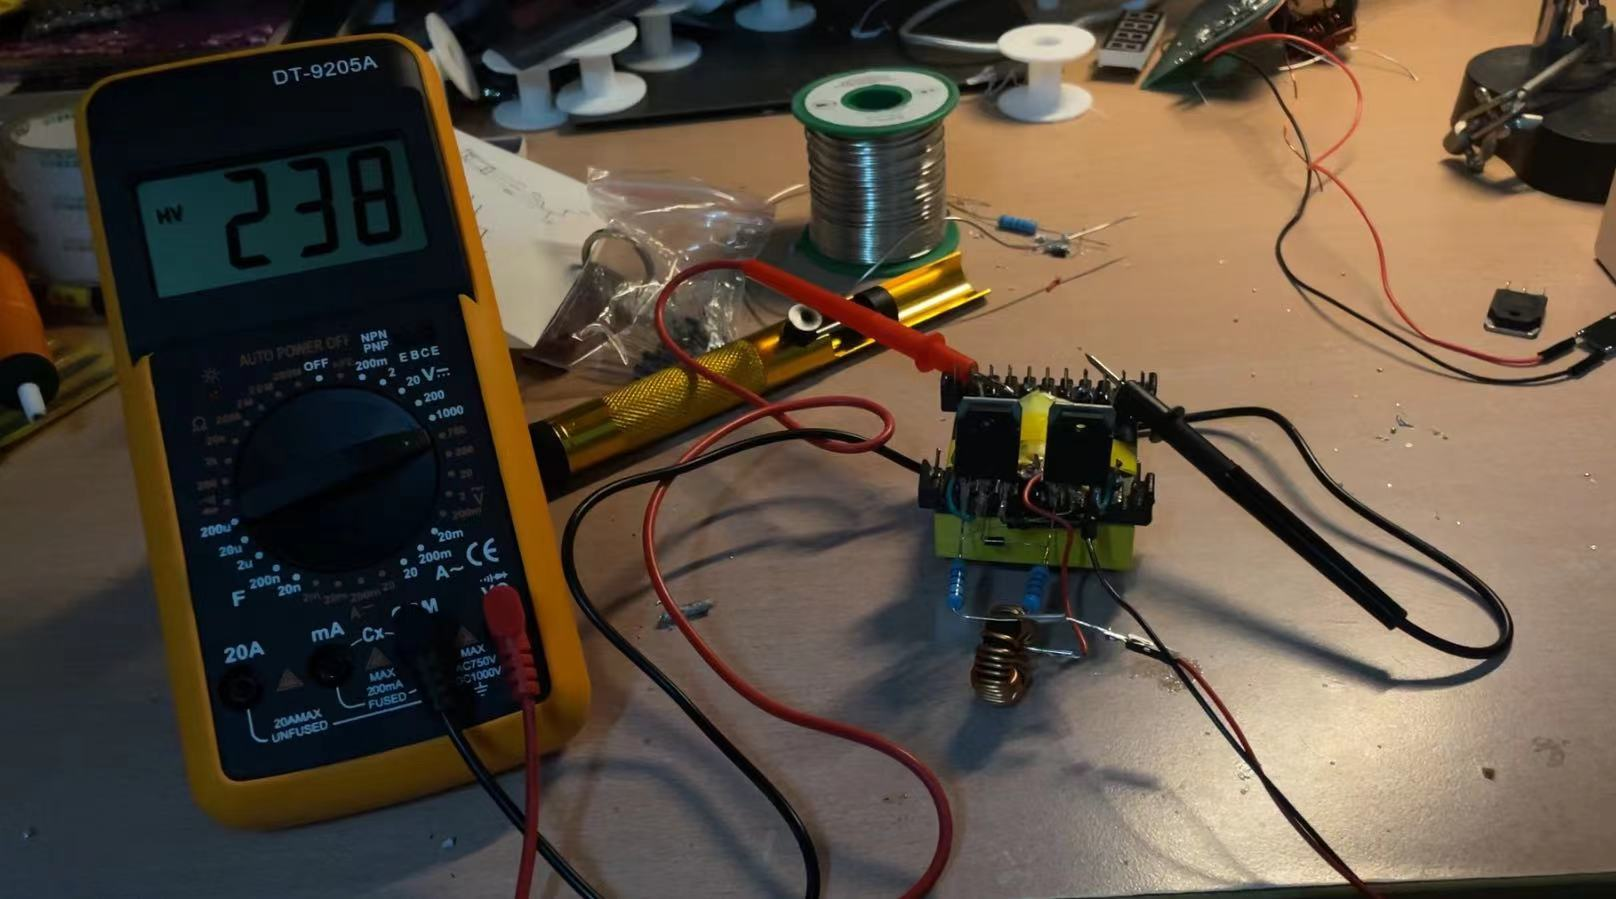
\includegraphics[width=\linewidth]{imgs/zvscircuit.jpg}
    \end{minipage}
    \begin{minipage}[b]{.45\linewidth}
        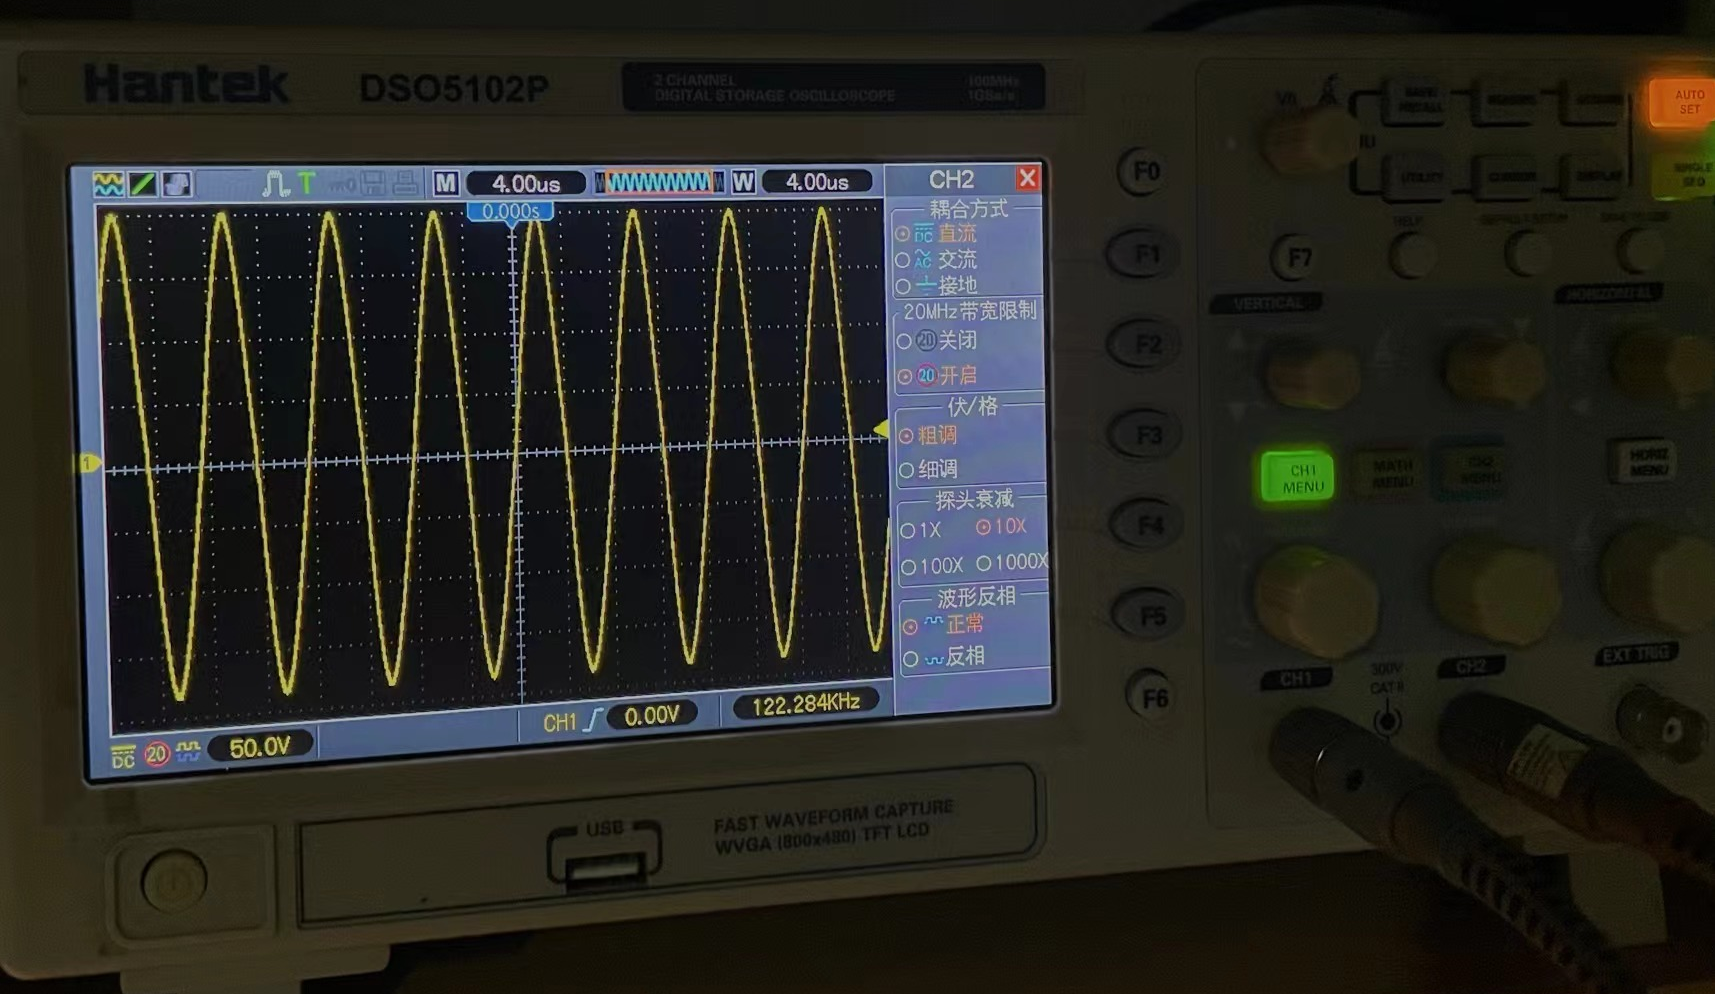
\includegraphics[width=\linewidth]{imgs/zvswave.png}
    \end{minipage}
    \caption{基于ZVS的升压电路-理论验证}
    \label{zvs}
\end{figure}
为了引入单片机的控制,我们采用一个\texttt{GPIO}引脚通过光耦隔离控制一只场管下拉ZVS电路低电平的方式,实现了电路的控制。电路的工作原理和实物图如图 \ref{zvs1} 所示。
\begin{figure}
    \centering
    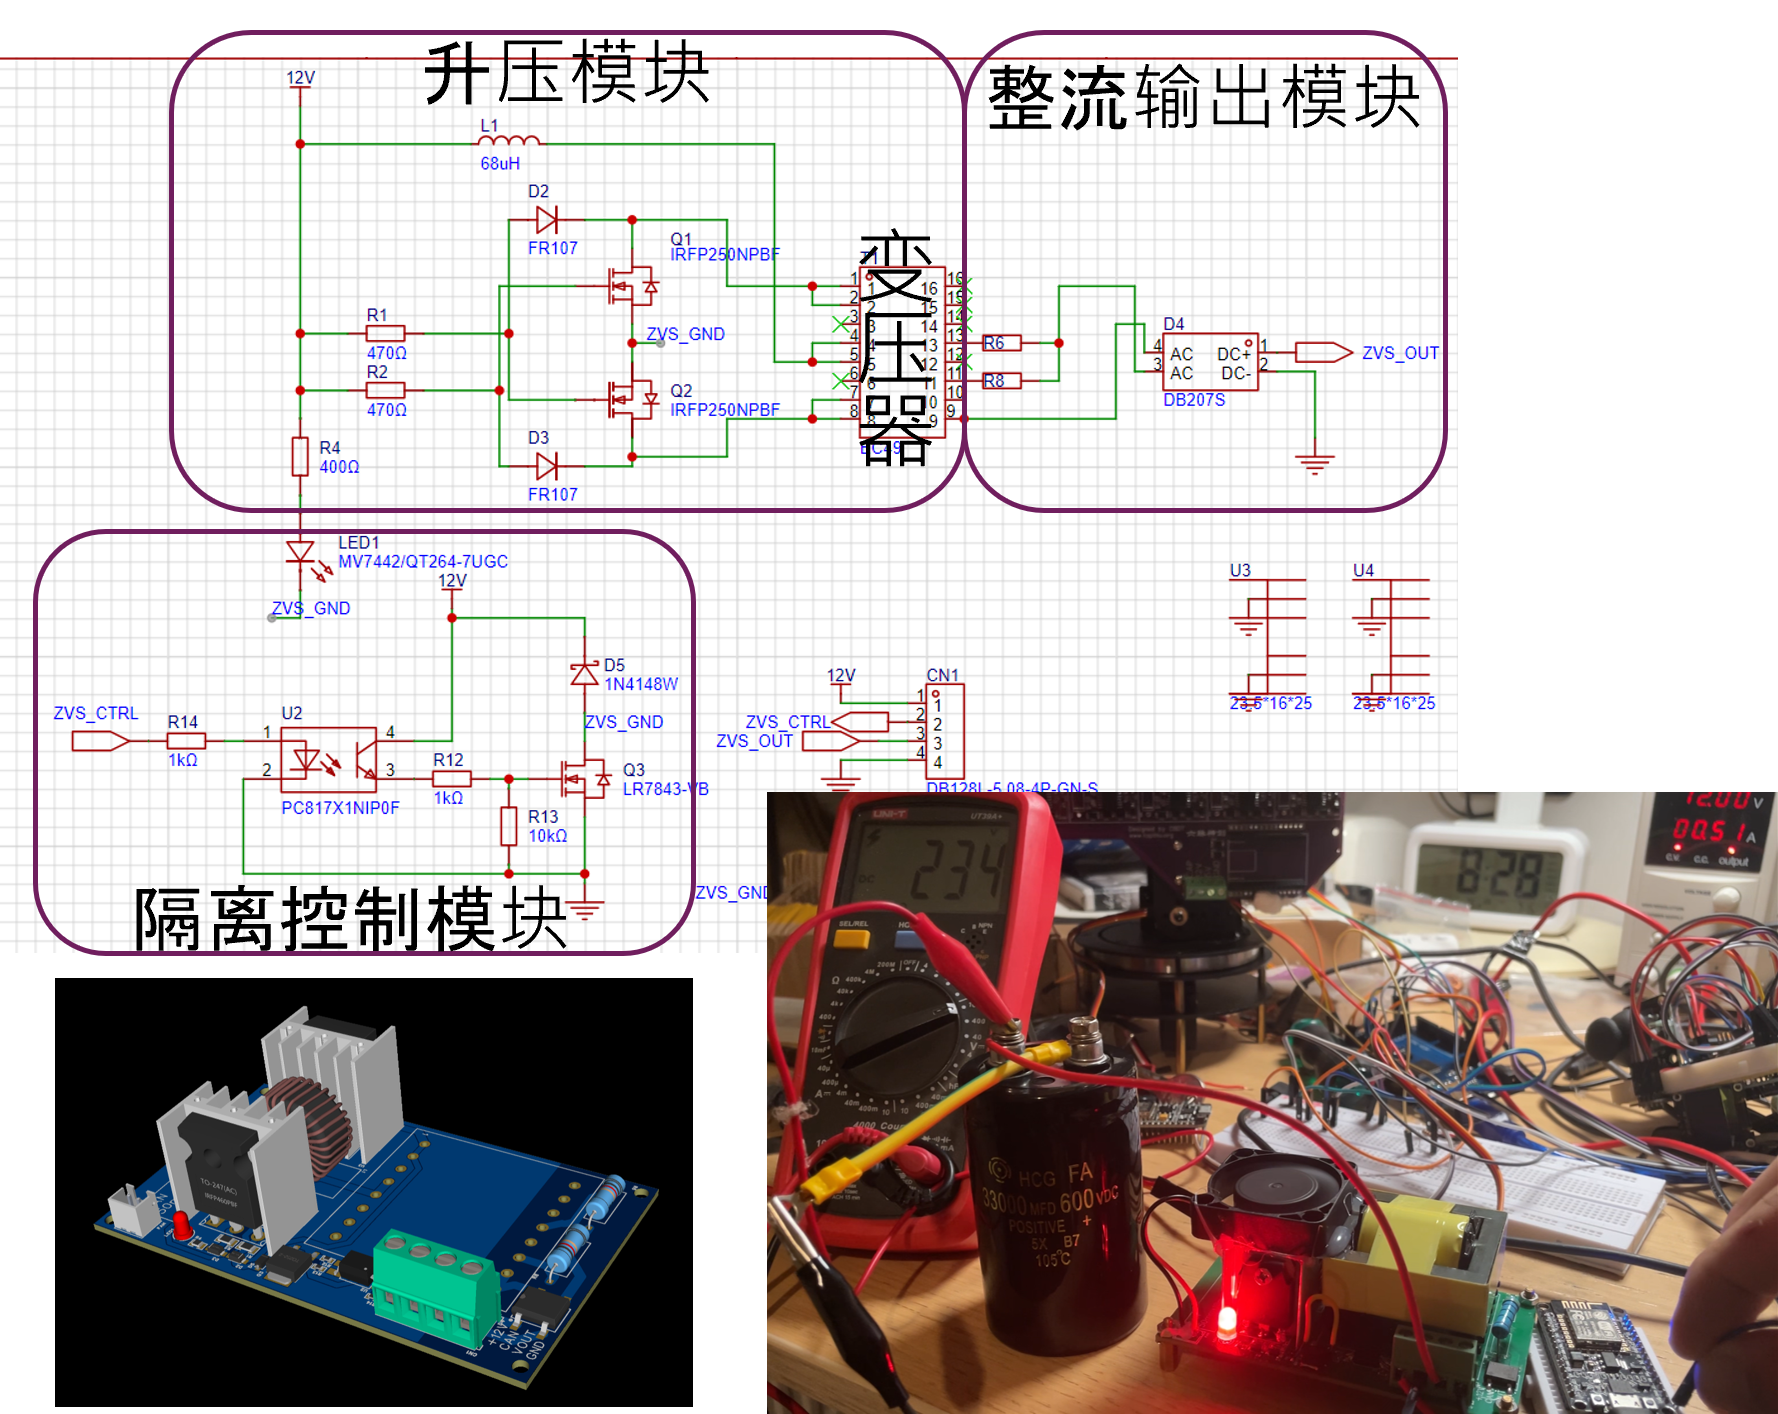
\includegraphics[width=.9\linewidth]{imgs/zvsmake.png}
    \caption{基于ZVS的升压电路-实物图}
    \label{zvs1}
\end{figure}
\subsection{多级线圈驱动电路}
为了实现电磁炮的线圈驱动,本项目采用半桥拓扑的线圈驱动电路。该电路利用两只场效应管和两只二极管,实现了对线圈的高效能量传输和能量回收。

根据基本电磁学知识不难知道,对于一个内外径分别为$r_1$和$r_2$的螺线管,其轴线上磁场强度$H$与电流$I$的关系为
\begin{equation}
    H(z)=\frac{NI}{2LR}\left[ (z+a)\ln \left(\frac{r_2+\sqrt{(z+a)^2+r_2^2}}{r_1+\sqrt{(z+a)^2+r_1^2}}\right)-(z-a)\ln \left(\frac{r_2+\sqrt{(z-a)^2+r_2^2}}{r_1+\sqrt{(z-a)^2+r_1^2}}\right)\right]
\end{equation}
从而根据虚功原理,不难求得子弹的受力大小为
\begin{equation}
    F=\frac{\partial W}{\partial z}=\frac{\partial\iiint_V\omega dV}{\partial z}\\
    \approx\frac{1}{2}\pi R^2B_m(H_{top}-H_{bottom})
\end{equation}
考虑到本次使作炮弹的A3钢的饱和磁感应强度为1.0T量级,采用python进行数值模拟,得到了炮弹在磁场中的受力曲线,如图 \ref{coil} 所示。

\begin{figure}
    \centering
    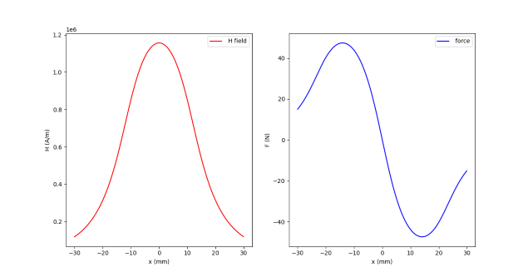
\includegraphics[width=.9\linewidth]{imgs/coid.png}
    \caption{线圈磁场力曲线}
    \label{coil}
\end{figure}
可以观察到,只要让炮弹“卡”在运动的磁力波第一个波峰之后处,就可以直接利用时序控制的方式实现炮弹的加速。此时的磁场力与炮弹位置负相关,形成了相对稳定的负反馈,因此使用有一定误差的线圈驱动电路也可以实现较好的加速效果。

我们设计半桥拓扑的线圈驱动电路,如图 \ref{igbt} 所示。
\begin{figure}
    \centering
\begin{minipage}[b]{.45\linewidth}
    \centering
    \begin{circuitikz}
    \draw(0,0)to[D=$D_1$](0,2);
    \draw(0,2)node[nigbt,anchor=E](Q1){Q1};
    \draw(2,0)node[nigbt,anchor=E](Q2){Q2};
    \draw(Q2.C)to[D=$D_2$](2,4);
    \draw(Q1.C)to[short](0,4);
    \draw(0,4)to[short](5,4);
    \draw(0,0)to[short](5,0);
    \draw(4,4)to[C,l_=$C_1$](4,0);
    \draw(0,2)to[L=$coil$](2,2);
    \draw(5,0)to[D,l_=$D_3$](5,4);
    \end{circuitikz}
\end{minipage}
\begin{minipage}[b]{.45\linewidth}
    \centering
    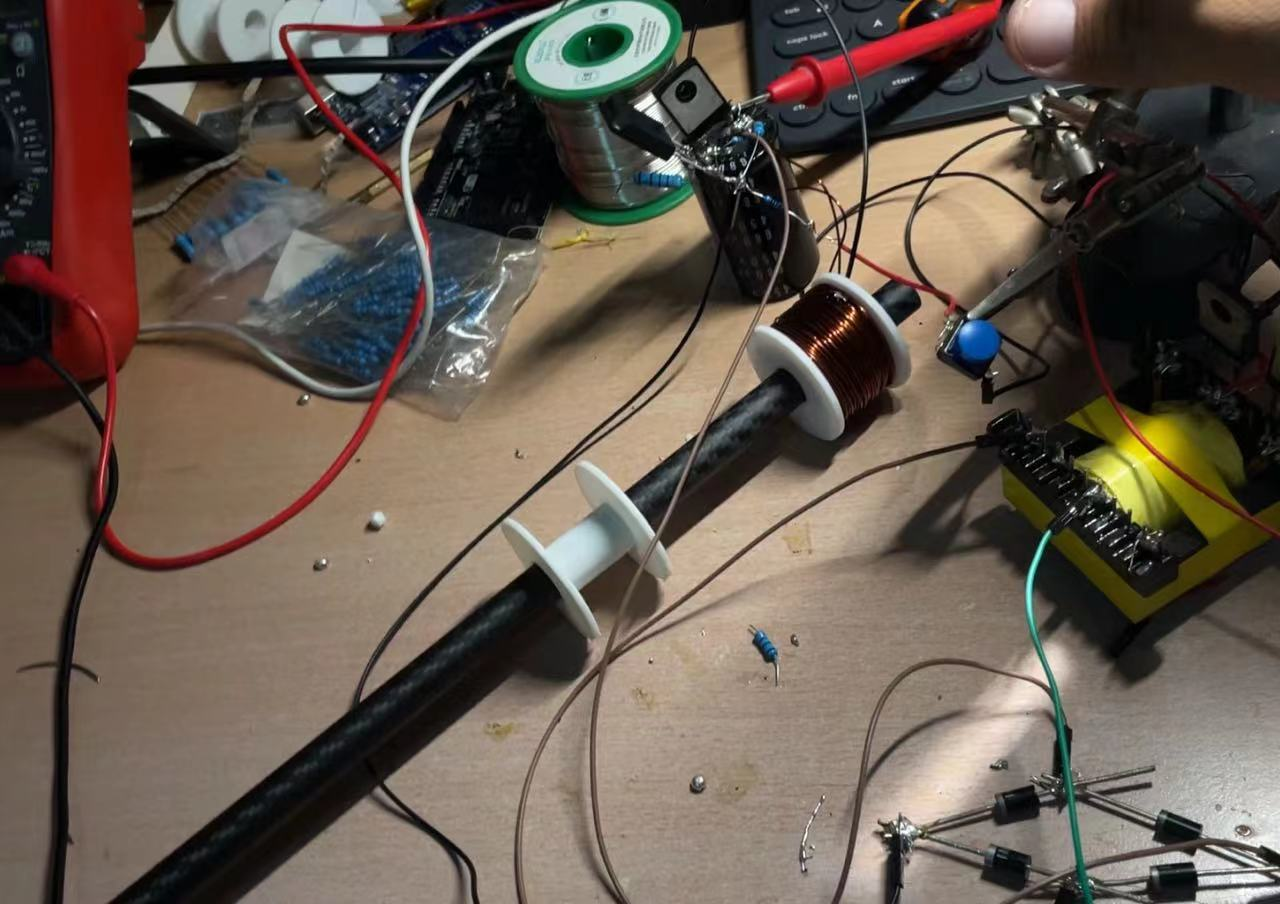
\includegraphics[width=.8\linewidth]{imgs/igbtcircuit.jpg}
\end{minipage}
\\
\hspace{20pt}
\\
\begin{minipage}[b]{.9\linewidth}
    \centering
    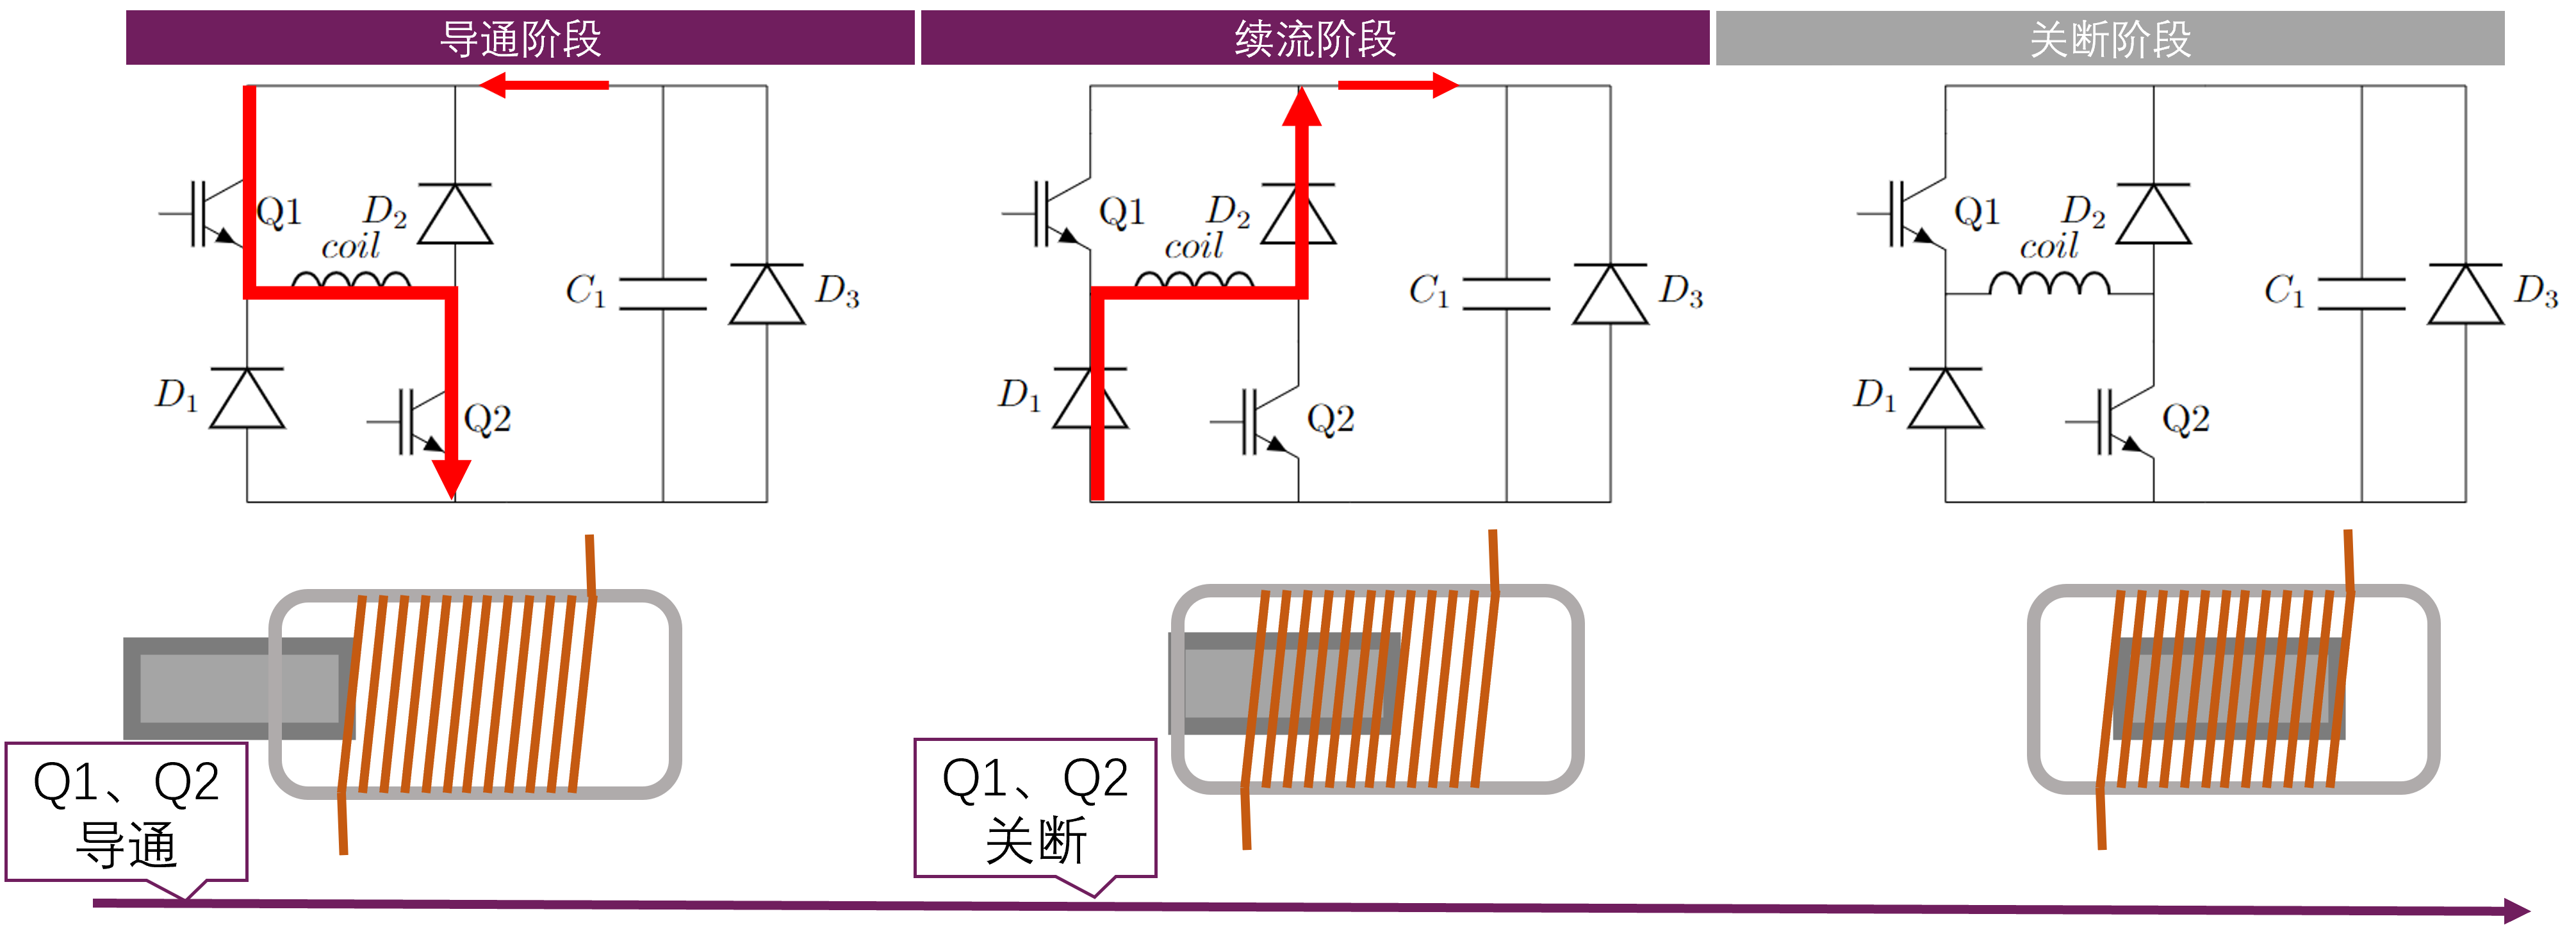
\includegraphics[width=.9\linewidth]{imgs/coiltime.png}
\end{minipage}
\caption{半桥IGBT驱动电路示意及单级测试}
\label{igbt}
\end{figure}

完成单级测试后,打样PCB得到了六级线圈的控制板,如图 \ref{coilpcb} 所示。

\begin{figure}
    \centering
    \includegraphics[width=.9\linewidth]{imgs/pcb.png}
    \caption{线圈驱动电路PCB}
    \label{coilpcb}
\end{figure}
\subsection{瞄准系统}
为了实现电磁炮的瞄准功能,本项目采用\texttt{Arduino Mega}控制舵机云台,实现了目标的自动瞄准和跟踪。人体识别基于部署在\texttt{K210}端侧计算平台的\texttt{YOLO2}模型进行人体识别,并返回目标位置和大小信息。

\section{系统全貌}
系统组装后的全貌如图 \ref{system} 所示。
\begin{figure}
    \centering
    \includegraphics[width=.9\linewidth]{imgs/sys.png}
    \caption{系统全貌}
    \label{system}
\end{figure}
本项目的硬件架构主要包括Arduino Mega、舵机云台、线圈驱动板、ESP8266、K210、ESP32、OLED屏幕、按钮、摇杆模块、充电宝和12V20A电源等。Arduino Mega作为主控单元,负责接收传感器数据、控制舵机云台和线圈驱动板,并与K210和ESP32进行通信。舵机云台用于瞄准目标,线圈驱动板用于驱动线圈,ESP8266用于实现遥控功能,K210用于人体识别,ESP32用于连接OLED屏幕和按钮,OLED屏幕用于显示系统状态,按钮和摇杆模块用于用户交互,充电宝和12V20A电源用于为系统供电。
\section{总结与展望}
本项目实现了智能电磁炮的基本功能,在电路、功能设计等方面得到了较好的效果。但本项目仍有较多的改进空间,横向和纵向上都有大量可供我们继续开发的方向。

横向上还可以探索外设传感器和用户界面,例如超声波传感器、红外传感器、触摸屏等,以丰富电磁炮的功能和应用场景。

纵向上则可以探索线圈的最优几何构型和电路拓扑,例如多线圈结构、多相驱动电路等,从而提高电磁炮的性能和效率。此外,探索更高效的充电器设计,可以提高电磁炮的续航能力。
\appendix
\section{软件源码清单}
\subsection{MEGA主控代码}
\begin{lstlisting}[language=C,caption=main.c]
    /**
    * @file main.cpp
    * @author WeitaoJiang cbdt.topthu.org
    * @brief
    * @version 0.1
    * @date 2024-08-10
    *
    * @copyright Copyright (c) 2024
    *
    */
   
   #include <Arduino.h>
   #include <Servo.h>
   #include <SPI.h>
   #include <RF24.h>
   #include <nRF24L01.h>
   #define IDLE_MODE 2
   #define RC_MODE 0
   #define AIM_MODE 1
   #define DEBUG_MODE -1
   #define K210 Serial2
   #define ESP8266 Serial1
   
   bool with_K210 = true;
   bool Use_RC = true;
   
   #define LASER_PIN 22
   #define CHARGE_ENA_PIN 37
   #define CHARGE_VOLTAGE_PIN A0
   
   #define ANALOG_TO_VOLTAGE_MULTIPLIER (300 / 800.0)
   typedef int switchmode_t;
   switchmode_t mode = IDLE_MODE;
   
   const int STAGE_CTRL_PINS[] = {38, 40, 42, 44, 46, 48};
   const int INIT_PIN = 32;
   const float aim_point_relative_x = 0.45;
   const float aim_point_relative_y = 0.5;
   
   Servo waist_servo, tilt_servo, load_servo;
   
   // servo.write(servo.read()+ Kp * err + Ki * int + Kd * diff);
   /*PID const configurations*/
   // waist
   const float Kp_waist = 0.3;
   const float Ki_waist = 0.0;
   const float Kd_waist = 0.05;
   // tilt
   const float Kp_tilt = 0.4;
   const float Ki_tilt = 0.0;
   const float Kd_tilt = 0.1;
   
   float int_waist = 0;
   float diff_waist = 0;
   float err_waist = 0;
   
   float int_tilt = 0;
   float diff_tilt = 0;
   float err_tilt = 0;
   
   // servo angle ctrl
   int load_angle = 100;
   int load_rest_angle = 10;
   
   struct Cmd
   {
     switchmode_t mode;
     int joy_x;
     int joy_y;
     int joy_btn_pressed;
   } cmd;
   /*PID functions*/
   float PID_waist(float err_)
   {
   
     int_waist += err_;
     diff_waist = err_ - err_waist;
     err_waist = err_;
     float ret = (Kp_waist * err_waist + Ki_waist * int_waist + Kd_waist * diff_waist) * 90.0;
     if (ret > 10)
       return 10;
     if (ret < -10)
       return -10;
     return ret;
   }
   float PID_tilt(float err_)
   {
   
     int_tilt += err_;
     diff_tilt = err_ - err_tilt;
     err_tilt = err_;
     return (Kp_tilt * err_tilt + Ki_tilt * int_tilt + Kd_tilt * diff_tilt) * 80.0;
   }
   
   void aim_target_1_itr(int target_x, int target_y, int canvas_width, int canvas_height)
   {
     int current_waist_angle = waist_servo.read();
     int current_tilt_angle = tilt_servo.read();
   
     float now_err_waist = -(target_x - canvas_width * aim_point_relative_x) / (float)canvas_width;
     float now_err_tilt = -(target_y - canvas_height * aim_point_relative_y) / (float)canvas_height;
   
     int delta_waist = PID_waist(now_err_waist);
     int delta_tilt = PID_tilt(now_err_tilt);
   
     waist_servo.write(current_waist_angle + delta_waist);
     tilt_servo.write(current_tilt_angle + delta_tilt);
     delay(20);
     waist_servo.write(waist_servo.read());
     tilt_servo.write(tilt_servo.read()); // protections
   }
   
   /*fire related funcs*/
   
   int VSETlo = 335;
   int VSEThi = VSETlo + 3; // voltage set points, sadly our zvs cant pid
   
   int stage_delay_us_arr[] = {0, 0, 0, 0, 0, 0};                // delay after stage
   long int stage_hold_us_arr[] = {1750, 800, 600, 420, 100, 0}; // hold time
   
   void fire()
   {
     digitalWrite(CHARGE_ENA_PIN, LOW);
     load_servo.write(load_rest_angle);
     delay(200);
     load_servo.write(load_angle);
     delay(200);
     for (int i = 0; i < 6; i++)
     {
       if (stage_hold_us_arr[i] == 0)
         continue;
       delayMicroseconds(stage_delay_us_arr[i]);
       digitalWrite(STAGE_CTRL_PINS[i], HIGH);
       delayMicroseconds(stage_hold_us_arr[i]);
       digitalWrite(STAGE_CTRL_PINS[i], LOW);
     }
     load_servo.write(load_rest_angle);
   }
   
   int get_voltage()
   {
     return analogRead(CHARGE_VOLTAGE_PIN) * ANALOG_TO_VOLTAGE_MULTIPLIER;
   }
   
   void update_charger()
   {
     // if (Use_RC)
     // {
     //   ESP8266.print("Voltage:");
     //   ESP8266.print(get_voltage());
     //   ESP8266.println(",Charging:1,Active:1");
     // }
     if (get_voltage() < VSETlo)
     {
       digitalWrite(CHARGE_ENA_PIN, HIGH);
     }
     else if (get_voltage() > VSEThi)
     {
       digitalWrite(CHARGE_ENA_PIN, LOW);
     }
     Serial.print("charging:");
     Serial.println(get_voltage());
     delay(100);
   }
   /*ctrl related funcs*/
   
   float JOY_X_TO_WAIST = 10.0 / 4096.0;
   float JOY_Y_TO_TILT = 5.0 / 4096.0;
   int read_human_sensor()
   {
     return 1;
   }
   
   void alarm()
   {
     // Serial.println("Human detected!");
     return; // todo: implement this function
   }
   
   /* MAIN */
   void setup()
   {
     // put your setup code here, to run once:
   
     Serial.begin(9600);
     Serial.println("Hello,world!");
     delay(1000);
     if (with_K210)
       K210.begin(9600);
     if (Use_RC)
       ESP8266.begin(9600);
     waist_servo.attach(7);
     waist_servo.write(155);
     tilt_servo.attach(3);
     tilt_servo.write(92);
     load_servo.attach(2);
   
     load_servo.write(load_rest_angle);
     delay(1000);
     pinMode(LASER_PIN, OUTPUT);
     pinMode(CHARGE_ENA_PIN, OUTPUT);
     pinMode(CHARGE_VOLTAGE_PIN, INPUT);
     for (int i = 0; i < 6; i++)
     {
       pinMode(STAGE_CTRL_PINS[i], OUTPUT);
     }
     pinMode(INIT_PIN, OUTPUT);
     delay(1000);
     Serial.println("init...");
     delay(1000);
     digitalWrite(INIT_PIN, HIGH);
     delay(1000);
     digitalWrite(INIT_PIN, LOW);
   }
   
   void loop()
   {
     update_charger();
     if (Use_RC && ESP8266.available())
     {
       String command = ESP8266.readStringUntil('\n');
       Serial.print("ESP says:");
       Serial.println(command);
       cmd.joy_btn_pressed = 0;
       sscanf(command.c_str(), "Mode:%d,JoyX:%d,JoyY:%d,JoyBtnPressed:%d", &cmd.mode, &cmd.joy_x, &cmd.joy_y, &cmd.joy_btn_pressed);
     }
     if (Use_RC == false)
     {
       cmd.mode = DEBUG_MODE;
     }
     switch (cmd.mode)
     {
   
     case DEBUG_MODE:
   
       delay(200);
       if (Serial.available())
       {
         String command = Serial.readString();
         if (command.indexOf("fire") != -1)
         {
           Serial.println("got:fire!");
           fire();
         }
       }
       break;
     case AIM_MODE:
       if (true)
       {
         int times_not_found = 0;
         alarm();
         digitalWrite(LASER_PIN, HIGH);
         while (read_human_sensor())
         {
           if (Use_RC && ESP8266.available())
           {
             String command = ESP8266.readStringUntil('\n');
             Serial.print("ESP says:");
             Serial.println(command);
             cmd.joy_btn_pressed = 0;
             sscanf(command.c_str(), "Mode:%d,JoyX:%d,JoyY:%d,JoyBtnPressed:%d", &cmd.mode, &cmd.joy_x, &cmd.joy_y, &cmd.joy_btn_pressed);
             if (cmd.mode == RC_MODE)
             {
               break;
             }
           }
           /*charge and check*/
           update_charger();
           if (!with_K210)
             delay(1000);
           /*read from K210 and aim.*/
           // K210.write("get");
           if (with_K210 && K210.available())
           {
             String text = String(K210.readStringUntil('\n'));
   
             delay(10);
             Serial.println(text);
             if (text.indexOf("target not found") != -1)
             {
               times_not_found++;
               if (times_not_found > 10)
               {
   
                 Serial.println("Target not found for 10 times, stop aiming.");
                 /*set angle to (90,30)*/
   
                 while (tilt_servo.read() > 90)
                 {
                   tilt_servo.write(tilt_servo.read() - 1);
                   delay(40);
                 }
                 while (tilt_servo.read() < 90)
                 {
                   tilt_servo.write(tilt_servo.read() + 1);
                   delay(40);
                 }
                 while (waist_servo.read() > 155)
                 {
                   waist_servo.write(waist_servo.read() - 1);
                   delay(40);
                 }
                 while (waist_servo.read() < 155)
                 {
                   waist_servo.write(waist_servo.read() + 1);
                   delay(40);
                 }
                 /*set pid vars to 0*/
                 int_waist = 0;
                 diff_waist = 0;
                 err_waist = 0;
                 int_tilt = 0;
                 diff_tilt = 0;
                 err_tilt = 0;
   
                 int tmp_var_waist = -20;
                 int tmp_var_tilt = -10;
                 /*start searching for target
                  waist: 140~160 160-(20~0)
                   tilt: 90~120 120-(30~0)
                 */
                 //(140,160)
                 while (true)
                 {
                   if (Use_RC && ESP8266.available())
                   {
                     String command = ESP8266.readStringUntil('\n');
                     Serial.print("ESP says:");
                     Serial.println(command);
                     cmd.joy_btn_pressed = 0;
                     cmd.joy_btn_pressed=0;
                     sscanf(command.c_str(), "Mode:%d,JoyX:%d,JoyY:%d,JoyBtnPressed:%d", &cmd.mode, &cmd.joy_x, &cmd.joy_y, &cmd.joy_btn_pressed);
                     if(cmd.joy_btn_pressed)
                     {
                       if (get_voltage() > VSETlo)
                       {
                         fire();
                       }
                     }
                     if (cmd.mode == RC_MODE)
                     {
                       break;
                     }
                   }
                   update_charger();
                   text = String(K210.readStringUntil('\n'));
                   Serial.println("searching for target,got: " + text);
                   if (text.indexOf("aim:") != -1)
                   {
                     int target_x, target_y, canvas_width, canvas_height, target_size;
                     sscanf(text.c_str(), "aim: %d %d canvas: %d %d size: %d", &target_x, &target_y, &canvas_width, &canvas_height, &target_size);
                     aim_target_1_itr(target_x, target_y, canvas_width, canvas_height);
                     times_not_found = 0;
                     break;
                   }
                   tilt_servo.write(100 - abs(tmp_var_tilt));
                   waist_servo.write(175 - abs(tmp_var_waist));
                   tmp_var_waist += 1;
                   tmp_var_tilt += 1;
                   if (tmp_var_waist > 20)
                   {
                     tmp_var_waist = -20;
                   }
                   if (tmp_var_tilt > 10)
                   {
                     tmp_var_tilt = -10;
                   }
                   delay(100);
                 }
                 continue;
               }
             }
             if (text.indexOf("aim:") != -1)
             {
               int target_x, target_y, canvas_width, canvas_height, target_size;
               sscanf(text.c_str(), "aim: %d %d canvas: %d %d size: %d", &target_x, &target_y, &canvas_width, &canvas_height, &target_size);
               aim_target_1_itr(target_x, target_y, canvas_width, canvas_height);
               times_not_found = 0;
             }
             // delay(50);
           }
         }
       }
       break;
     case RC_MODE:
       if (cmd.joy_btn_pressed)
       {
         if (get_voltage() > VSETlo)
         {
           fire();
         }
       }
   
       break;
     }
   }
\end{lstlisting}   
\subsection{K210端代码}
\begin{lstlisting}[language=python,caption=main.py]
from machine import UART,Timer
from fpioa_manager import fm
import sensor, image, time, lcd
from maix import KPU
import gc



fm.register(6,fm.fpioa.UART1_RX,force=True)
fm.register(7,fm.fpioa.UART1_TX,force=True)

uart1 = UART(UART.UART1, 9600)
uart1.write('Hello From K210!')
lcd.init()

sensor.reset()
sensor.set_vflip(1)                 
sensor.set_hmirror(1)               

sensor.set_pixformat(sensor.RGB565) # Set pixel format to RGB565 (or GRAYSCALE)
sensor.set_framesize(sensor.QVGA)   # Set frame size to QVGA (320x240)
sensor.skip_frames(time = 1000)     # Wait for settings take effect.
clock = time.clock()                # Create a clock object to track the FPS.
od_img = image.Image(size=(320,256))


anchor_body_detect = (0.0978, 0.1758, 0.1842, 0.3834, 0.3532, 0.5982, 0.4855, 1.1146, 0.8869,
                        1.6407, 1.2388, 3.4157, 2.0942, 2.1114, 2.7138, 5.0008, 6.0293, 6.4540)
body_kpu = KPU()

body_kpu.load_kmodel("/sd/uint8_person_detect_v1_old.kmodel")

body_kpu.init_yolo2(anchor_body_detect, anchor_num=9, img_w=320, img_h=240, net_w=320 ,
                    net_h=256 ,layer_w=10 ,layer_h=8, threshold=0.7, nms_value=0.2, classes=1)
aim_x = -1
aim_y = -1
body_size = -1
while True:
    gc.collect()
    clock.tick()                    # Update the FPS clock.
    img = sensor.snapshot()
    a = od_img.draw_image(img, 0,0)
    od_img.pix_to_ai()

    body_kpu.run_with_output(od_img)
    body_boxes = body_kpu.regionlayer_yolo2()
    if len(body_boxes) > 0:


        for l in body_boxes :
            aim_x = int(l[0]+l[2]/2)
            aim_y = int(l[1]+l[3]*0.5)
            body_size = l[2]*l[3]
            a = img.draw_rectangle(l[0],l[1],l[2],l[3], color=(255, 0, 0),thickness=2)
            img.draw_cross(int(l[0]+l[2]/2),int(l[1]+l[3]*0.5),color=(255,255,255),size=10,thickhess=1)
    else:
        aim_x = -1
        aim_y = -1
        body_size = -1
    if aim_x >= 0 and aim_y >= 0:
        uart1.write("aim: "+str(aim_x)+" "+str(aim_y)+" canvas: "+str(od_img.width())+" "+str(od_img.height())+" size: "+ str(body_size)+'\n')
    else:
        uart1.write("target not found\n")
    fps = clock.fps()
    a = img.draw_string(0, 0, "%2.1ffps" %(fps), color=(0, 60, 128), scale=2.0)
    lcd.display(img)
body_kpu.deinit()
    
\end{lstlisting}
\subsection{ESP8266/ESP32端代码}
\begin{lstlisting}[language=C,caption=esp8266.ino]
    #include<ESP8266WiFi.h>
    #include <WiFiClient.h>
    #include <WiFiServer.h>
    #include<Arduino.h>
    #include<HardwareSerial.h>
    #include<stdio.h>
    #include<string.h>
    
    #include<wl_definitions.h>
    
    const char* ssid="esp8266";
    const char* password="wtgg6666";
    const int port = 8080;
    
    WiFiServer server(port);
    
    void setup() {
      Serial.begin(9600);
      WiFi.softAP(ssid,password);
      //WiFi.begin(ssid,password);
      Serial.print("\nAccess Point: ");
      Serial.println(ssid);
      Serial.print("IP address: ");
      Serial.println(WiFi.softAPIP());
    
      //while (WiFi.status() != WL_CONNECTED) {
      //  delay(1000);
      //  Serial.print(".");
      //}
    
      //Serial.println("WiFi connected");
      //Serial.println("IP address: ");
      //Serial.println(WiFi.localIP());
    
      server.begin();
      Serial.println("Server started");
    
    }
    void loop() {
      WiFiClient client = server.available(); 
      if (client) { 
        //Serial.println("New client connected");
        //delay(2000);
        if(Serial.available()){
          /*Serial.println("Voltage:");
          delay(1000);
          int voltage=Serial.read();
          Serial.println("Charging?:");
          delay(1000);
          bool charging=Serial.read();
          Serial.println("Active?:");
          delay(1000);
          bool active=Serial.read();
          */
          char* chpr=new char[100];
          sprintf(chpr,Serial.readStringUntil('\n').c_str());
          //sprintf(chpr,"Voltage:%d,Charging:%d,Active:%d",voltage,charging,active);
          client.println(chpr);
          Serial.print(chpr);
          delete chpr;
        }
        //client->server(->client)
        //int mode,joyx,joyy,joybtn;
        //int flag=-1;
        while (client.connected()) { 
          if (client.available()) {
            String line = client.readStringUntil('\n'); 
            //Serial.print("Received from client: ");
            Serial.println(line);
            //client.println(line);
            //flag=sscanf(line.c_str(),"Mode:%d,JoyX:%d,JoyY:%d,JoyBtnPressed:%d",mode,joyx,joyy,joybtn);
          }
        }
        client.stop();
        //Serial.println("Client disconnected");
        //delay(1000);
      }
    }
\end{lstlisting}
\begin{lstlisting}[language=C,caption=ESP32.ino]
    #include <WiFi.h>
    #include<Arduino.h>
    #include<HardwareSerial.h>
    #include<stdio.h>
    #include<stdlib.h>
    #include<string.h>
    #include<U8g2lib.h>
    U8G2_SSD1306_128X32_UNIVISION_F_HW_I2C u8g2(U8G2_R0, /* reset=*/ U8X8_PIN_NONE);
    
    //#include<wl_definitions.h>
    
    const char* ssid = "esp8266";
    const char* password = "wtgg6666";
    const char* host = "192.168.4.1";
    const int port = 8080; 
    const int Rx=32,Ry=33,SW=25;
    const int Btn=13;
    const int R=12,G=14,B=27;
    WiFiClient client;
    
    void draw1(void) {
      u8g2.setFont(u8g2_font_ncenB08_tr);
      u8g2.drawStr(16, 16, "Electromagnetic");
      u8g2.drawStr(40, 28, "Cannon");
    }
    void draw2(void) {
      u8g2.setFont(u8g2_font_ncenB08_tr); 
      u8g2.drawStr(32, 20, "Connected!");
    }
    void draw3(void) {
      u8g2.setFont(u8g2_font_ncenB08_tr);
      u8g2.drawLine(20,32,68,32);
      u8g2.drawLine(20,30,68,30);
      u8g2.drawLine(20,32,20,30);
      u8g2.drawLine(68,32,68,30);
      u8g2.drawLine(22,30,22,28);
      u8g2.drawLine(22,28,64,28);
      u8g2.drawLine(64,30,64,28);
      u8g2.drawLine(40,24,40,28);
      u8g2.drawLine(48,24,48,28);
      u8g2.drawLine(40,24,48,24);
      u8g2.drawLine(40,18,42,26);
      u8g2.drawLine(44,18,46,26);
      u8g2.drawLine(30,18,71,8);
      u8g2.drawLine(30,17,62,9);
      u8g2.drawLine(30,19,62,11);
      u8g2.drawLine(29,16,30,20);
      u8g2.drawLine(34,15,34,19);
      u8g2.drawLine(37,14,38,18);
      u8g2.drawLine(41,13,42,17);
      u8g2.drawLine(45,12,46,16);
      u8g2.drawLine(49,11,50,15);
      u8g2.drawLine(53,10,54,14);
      u8g2.drawLine(57,9,58,13);
      u8g2.drawLine(61,8,62,12);
      u8g2.drawLine(88,4,90,6);
      u8g2.drawLine(90,6,96,5);
      u8g2.drawLine(96,5,99,2);
      u8g2.drawLine(99,2,94,2);
      u8g2.drawLine(94,2,88,4);
      u8g2.drawLine(12,8,9,18);
      u8g2.drawLine(9,18,13,16);
      u8g2.drawLine(13,16,12,24);
      u8g2.drawLine(12,24,15,14);
      u8g2.drawLine(15,14,11,16);
      u8g2.drawLine(11,16,12,8);
      u8g2.drawStr(76,24,"Electrify!");
    }
    
    void setup() {
      Serial.begin(9600);
      WiFi.begin(ssid, password);
      pinMode(SW,INPUT_PULLUP);
      pinMode(Btn,INPUT);
      pinMode(Rx,INPUT);
      pinMode(Ry,INPUT);
      pinMode(R, OUTPUT);
      pinMode(G, OUTPUT);
      pinMode(B, OUTPUT);
      u8g2.begin();
      u8g2.firstPage();
      do {
        draw3();
      } while(u8g2.nextPage());
      delay(3000);
      u8g2.firstPage();
      do {
        draw1();
      } while(u8g2.nextPage());
      delay(2000);
    
      while (WiFi.status() != WL_CONNECTED) {
        delay(1000);
        Serial.print(".");
      }
    
      Serial.println("WiFi connected");
      Serial.println("IP address: ");
      Serial.println(WiFi.localIP());
    
    }
    
    int connection=0;
    int btn=0,btn_pre=0,btn_swch=0,btn_init=0;
    void loop() {
      if (!client.connect(host, port)) { 
        connection=0;
        digitalWrite(R,LOW);
        digitalWrite(G,LOW);
        digitalWrite(B,LOW);
        Serial.println("Connection to server failed");
    
        u8g2.firstPage();
        do {
          draw3();
        } while(u8g2.nextPage());
        delay(3000);
    
        u8g2.firstPage();
        do {
          draw1();
        } while(u8g2.nextPage());
        delay(2000);
        return;
      }
    
      if(connection==0){
        Serial.println("Connected to server");
        u8g2.firstPage();
        do {
          draw2();
        } while(u8g2.nextPage());
      }
      connection=1;
      
      int flag=-1,flag2=0;
      int voltage=0,charging=0,active=0;
      if (client.available()) { 
        String line = client.readStringUntil('\n');
        //Serial.print("Received from server: ");
        Serial.println(line);
        flag=sscanf(line.c_str(),"Voltage:%d,Charging:%d,Active:%d",&voltage,&charging,&active);
      }
      if(flag!=-1){
        int progress,progressX,progressWidth,progressHeight;
        u8g2.firstPage();
        do {
          u8g2.setFont(u8g2_font_ncenB08_tr);
          u8g2.setCursor(36, 8);
          if (charging == 0 && active == 1) {
            u8g2.print("Active");
          } 
          else if(charging == 1 && active == 0) {
            u8g2.print("Charging");
          }
          else {
            Serial.print("Error");
            flag2=1;
          }
          if(flag2==0){
            u8g2.setCursor(24, 16);
            u8g2.print("Voltage:");
    
            u8g2.setCursor(70, 16);
            u8g2.print(voltage);
            u8g2.print("V");
    
            progress = (int)(voltage / 3.0); 
            progressX = 14; 
            progressWidth = 100;
            progressHeight = 8; 
            u8g2.drawFrame(progressX, 22, progressWidth, progressHeight);
    
            if (progress > 0) {
              u8g2.drawBox(progressX, 22, progress, progressHeight);
            }
          }
        } while(u8g2.nextPage());
        flag=-1;
        flag2=0;
      }
    
      //client.println("Hello from ESP32 Client");
    
      int x=analogRead(Rx);
      int y=analogRead(Ry);
      int sw=1-digitalRead(SW);
      btn=digitalRead(Btn);
      btn_swch=abs(btn-btn_pre);
      btn_init+=btn_swch;
      btn_init%=4;
      //Serial.println(btn);//
      char* chtr=new char[100];
      sprintf(chtr,"Mode:%d,JoyX:%d,JoyY:%d,JoyBtnPressed:%d",btn_init/2,x,y,sw);
      client.println(chtr);
      //client.print("\n");
      Serial.println(chtr);
      //Serial.print("\n");
      digitalWrite(R,LOW);
      digitalWrite(G,LOW);
      digitalWrite(B,LOW);
      if(btn_init==0){
        digitalWrite(G,HIGH);
        delay(100);
      }
      else if(btn_init==2){
        digitalWrite(B,HIGH);
        delay(100);
      }
      else
      {
        digitalWrite(R,HIGH);
      }
    
      //client.println("ESP32 Client received your message");
    
      client.stop();
      //Serial.println("Client disconnected");
    
      btn_pre=btn;
    
      delay(200);
    }
\end{lstlisting}
\subsection{python仿真代码}
\begin{lstlisting}[language=Python,caption=force.py]
import math
from scipy.interpolate import interp1d  
import numpy as np
import pandas as pd  

from scipy.optimize import curve_fit  
import matplotlib.pyplot as plt  

bullet_len_mm = 22
bullet_rad_mm = 8/2
class Coil:  
    def __init__(self, location, length, N, innerRadius, outerRadius):  
        self.length = length     
        self.innerRadius = innerRadius 
        self.outerRadius = outerRadius  
        self.N = N                      
        self.u0 = 4 * math.pi * 1e-7     
    def HFieldCoil3(self, current, z):  
        L=self.length
        a=L/2
        r2=self.outerRadius
        r1=self.innerRadius
        R=r2-r1
        def logarithm(pos):  
            return pos * math.log((math.sqrt(pos ** 2 + r2 ** 2) + r2) /  
                                    (math.sqrt(pos ** 2 + r1 ** 2) + r1))  
            
        return ( self.N*current/(2*L*R) ) * (logarithm(z+a)-logarithm(z-a)) 
coil = Coil(0, 23.4*1e-3, 200, 0.5*12.4*1e-3, 0.5*40*1e-3)  
current = 200  
plt.figure(figsize=(10,10))
xx=[ pos for pos in np.arange(-30,30,0.1)]
yy=[ coil.HFieldCoil3( current, x*1e-3)   for x in xx]
Fyy = []
for i in range (0,len(xx)):
    Fyy.append((coil.HFieldCoil3( current, (xx[i]+bullet_len_mm/2)*1e-3)
                -coil.HFieldCoil3( current, (xx[i]-bullet_len_mm/2)*1e-3))
                *(bullet_rad_mm*1e-3)**2*math.pi)
plt.subplot(1,2,1)
plt.plot(xx, yy, color='red', label=' H field')  
plt.xlabel('x (mm)')  
plt.ylabel('H (A/m)')  
plt.legend()  
plt.subplot(1,2,2)
plt.plot(xx, Fyy, color='blue', label=' force')
plt.xlabel('x (mm)')
plt.ylabel('F (N)')
plt.legend()
plt.show()

\end{lstlisting}
\section{相关链接}
可点击
\href{https://www.bilibili.com/video/BV1nJpbeAEKk/?share_source=copy_web&vd_source=4597eff6ca01ce40fa5a055d7830e7c7}{视频链接}观看演示视频。

本项目开源,github仓库为\href{https://github.com/CBDT-JWT/autoE_Mgun}{此链接}。

\section{参考文献}
\begin{enumerate}
    \item 李小鹏,徐征,李立毅:《电磁线圈发射原理》,北京:兵器工业出版社,2019.
    \item 清华大学电力系高压技术专业编著.冲击大电流技术.北京:科学出版社,1978.139-141.
    \item 王莹,肖峰:《电炮原理》,1993.
    \item 李国林:《电子电路与系统基础》,北京:清华大学出版社,2020

\end{enumerate}
\end{document}